% #######################################
% ########### FILL THESE IN #############
% #######################################
\def\mytitle{Coursework 2 - Blog Application}
\def\mykeywords{Ciphers,HTML,CSS,JS,NODE,EXPRESS,MYSQL,BLOG,SET08101,NAPIER,UNIVERSITY}
\def\myauthor{David McCahon}
\def\contact{40214392@live.napier.ac.uk}
\def\mymodule{Module Title (SET08101)}
% #######################################
% #### YOU DON'T NEED TO TOUCH BELOW ####
% #######################################
\documentclass[10pt, a4paper]{article}
\usepackage[a4paper,outer=1.5cm,inner=1.5cm,top=1.75cm,bottom=1.5cm]{geometry}
\usepackage{graphicx}
\graphicspath{{./images/}}
%colour our links, remove weird boxes
\usepackage[colorlinks,linkcolor={black},citecolor={blue!80!black},urlcolor={blue!80!black}]{hyperref}
%Stop indentation on new paragraphs
\usepackage[parfill]{parskip}
%% Arial-like font
\IfFileExists{uarial.sty}
{
    \usepackage[english]{babel}
    \usepackage[T1]{fontenc}
    \usepackage{uarial}
    \renewcommand{\familydefault}{\sfdefault}
}{
    \GenericError{}{Couldn't find Arial font}{ you may need to install 'nonfree' fonts on your system}{}
    \usepackage{lmodern}
    \renewcommand*\familydefault{\sfdefault}
}
%Napier logo top right
\usepackage{watermark}
%Lorem Ipusm dolor please don't leave any in you final report ;)
\usepackage{lipsum}
\usepackage{xcolor}
\usepackage{listings}
%give us the Capital H that we all know and love
\usepackage{float}
%tone down the line spacing after section titles
\usepackage{titlesec}
%Cool maths printing
\usepackage{amsmath}
%PseudoCode
\usepackage{algorithm2e}

\titlespacing{\subsection}{0pt}{\parskip}{-3pt}
\titlespacing{\subsubsection}{0pt}{\parskip}{-\parskip}
\titlespacing{\paragraph}{0pt}{\parskip}{\parskip}
\newcommand{\figuremacro}[5]{
    \begin{figure}[#1]
        \centering
        \includegraphics[width=#5\columnwidth]{#2}
        \caption[#3]{\textbf{#3}#4}
        \label{fig:#2}
    \end{figure}
}

\lstset{
	escapeinside={/*@}{@*/}, language=C++,
	basicstyle=\fontsize{8.5}{12}\selectfont,
	numbers=left,numbersep=2pt,xleftmargin=2pt,frame=tb,
    columns=fullflexible,showstringspaces=false,tabsize=4,
    keepspaces=true,showtabs=false,showspaces=false,
    backgroundcolor=\color{white}, morekeywords={inline,public,
    class,private,protected,struct},captionpos=t,lineskip=-0.4em,
	aboveskip=10pt, extendedchars=true, breaklines=true,
	prebreak = \raisebox{0ex}[0ex][0ex]{\ensuremath{\hookleftarrow}},
	keywordstyle=\color[rgb]{0,0,1},
	commentstyle=\color[rgb]{0.133,0.545,0.133},
	stringstyle=\color[rgb]{0.627,0.126,0.941}
}

\thiswatermark{\centering \put(336.5,-38.0){
\includegraphics[scale=0.8]{logo}} }
\title{\mytitle}
\author{\myauthor\hspace{1em}\\\contact\\Edinburgh Napier University\hspace{0.5em}-\hspace{0.5em}\mymodule}
\date{}
\hypersetup{pdfauthor=\myauthor,pdftitle=\mytitle,pdfkeywords=\mykeywords}
\sloppy

\usepackage{color}
\definecolor{lightgray}{rgb}{.9,.9,.9}
\definecolor{darkgray}{rgb}{.4,.4,.4}
\definecolor{purple}{rgb}{0.65, 0.12, 0.82}
\lstdefinelanguage{JavaScript}{
  keywords={break, case, catch, continue, debugger, default, delete, do, else, false, finally, for, function, if, in, instanceof, new, null, return, switch, this, throw, true, try, typeof, var, void, while, with},
  morecomment=[l]{//},
  morecomment=[s]{/*}{*/},
  morestring=[b]',
  morestring=[b]",
  ndkeywords={class, export, boolean, throw, implements, import, this},
  keywordstyle=\color{blue}\bfseries,
  ndkeywordstyle=\color{darkgray}\bfseries,
  identifierstyle=\color{black},
  commentstyle=\color{purple}\ttfamily,
  stringstyle=\color{red}\ttfamily,
  sensitive=true
}

\lstset{
   language=JavaScript,
   extendedchars=true,
   showstringspaces=false,
   showspaces=false,
   numbers=left,
   numberstyle=\footnotesize,
   numbersep=9pt,
   tabsize=2,
   breaklines=true,
   showtabs=false,
   captionpos=b
}

\usepackage{enumitem,amssymb}
\newlist{todolist}{itemize}{2}
\setlist[todolist]{label=$\square$}
\usepackage{pifont}
\newcommand{\cmark}{\ding{51}}%
\newcommand{\xmark}{\ding{55}}%
\newcommand{\done}{\rlap{$\square$}{\raisebox{2pt}{\large\hspace{1pt}\cmark}}%
\hspace{-2.5pt}}
\newcommand{\wontfix}{\rlap{$\square$}{\large\hspace{1pt}\xmark}}

% #######################################
% ########### START FROM HERE ###########
% #######################################
\begin{document}    
\begin{titlepage} % Suppresses displaying the page number on the title page and the subsequent page counts as page 1
	\newcommand{\HRule}{\rule{\linewidth}{0.5mm}} % Defines a new command for horizontal lines, change thickness here
	
	\center % Centre everything on the page
	
	%------------------------------------------------
	%	Headings
	%------------------------------------------------
	
	\textsc{\LARGE}\\[1.5cm] % Main heading such as the name of your university/college
	
	\textsc{\Large SET08101}\\[0.5cm] % Major heading such as course name
	
	\textsc{\large Web Technologies}\\[0.5cm] % Minor heading such as course title
	
	%------------------------------------------------
	%	Title
	%------------------------------------------------
	
	\HRule\\[0.4cm]
	
	{\huge\bfseries Coursework 2 - Blog Application}\\[0.4cm] % Title of your document
	
	\HRule\\[1.5cm]
	
	%------------------------------------------------
	%	Author(s)
	%------------------------------------------------
	
	\begin{minipage}{0.4\textwidth}
		\begin{flushleft}
			\large
			\textit{Author}\\
			\textsc{David McCahon (40214392)} % Your name
		\end{flushleft}
	\end{minipage}

	
	% If you don't want a supervisor, uncomment the two lines below and comment the code above
	%{\large\textit{Author}}\\
	%John \textsc{Smith} % Your name
	
	%------------------------------------------------
	%	Date
	%------------------------------------------------
	
	\vfill\vfill\vfill % Position the date 3/4 down the remaining page
	
	{\large\today} % Date, change the \today to a set date if you want to be precise
	
	%------------------------------------------------
	%	Logo
	%------------------------------------------------
	
	%\vfill\vfill
	%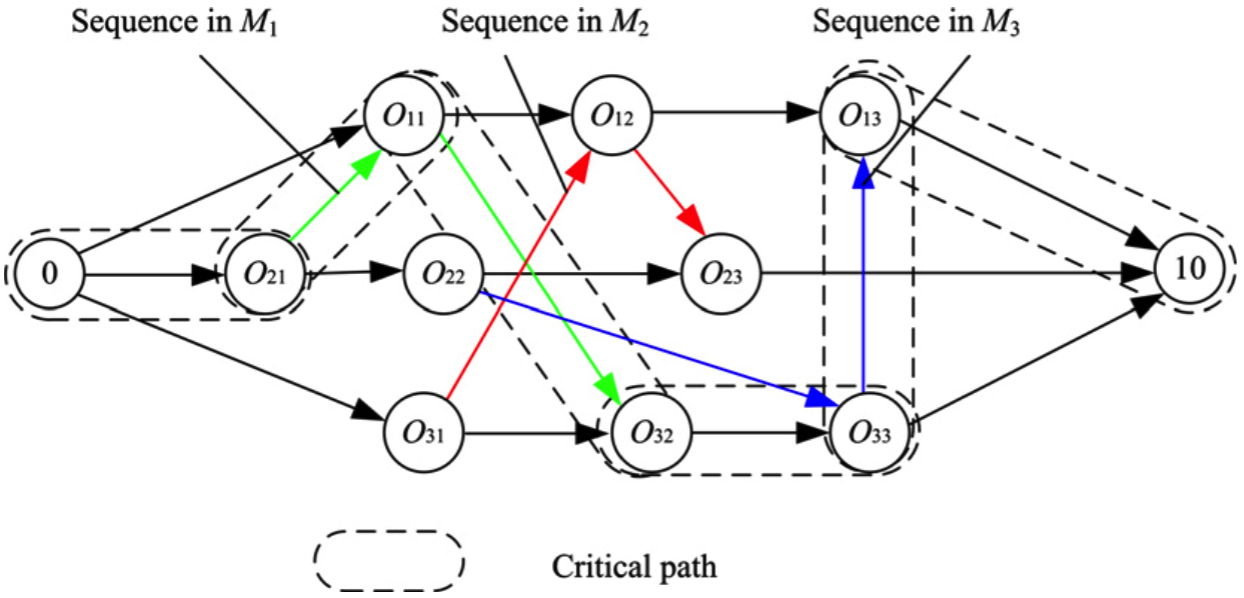
\includegraphics[width=0.2\textwidth]{placeholder.jpg}\\[1cm] % Include a department/university logo - this will require the graphicx package
	 
	%----------------------------------------------------------------------------------------
	
	\vfill % Push the date up 1/4 of the remaining page
	
\end{titlepage}

\tableofcontents  \pagebreak
    \section{Introduction}
  Within today's society people are easily offended.  With a world full of offended people, feelings run high and people require a place to post their thoughts, opinions and reasoning that are going on within their day to day life. 

A blog is the perfect way for users to post their personal views for the world to see.  Blogs allow for a variety of method flexible and defined to the users interests, topics and variety of posts
that they may wish to share. 

It is important that the user is able to create, edit, update and delete posts that they make.  For example, a controversial post on their blog may receive a negative response and the user may wish to either update their post or delete it all together. 

This application will use HTML, CSS, NodeJ, EJS and MYSQL  to create a functional blog which is accessible by multiple users which could be used in a variety of ways. 

A simplistic design will be used to enhance user experience.  Clear instructions will be provided on how to use the blog as buttons and hyperlinks are clearly marked on their meaning.  For example, "Create Post", "Edit", "Delete" clearly mark out the intended purpose of the function.
    
	
	\section{Software Design}
	The design of the webpage aims to give the user a good experience.  This includes efficient color schemes to make the application feel pleasant, easy to read text and clear instructions of international  buttons found within the application. 
	
	\subsection{Approach}
	The following languages will be used to code the website alongside their usage;\\
	\textbf{1. HTML} - HTML will be used to provide the structure of the application.  This includes setting out headers, footers, containers and dividers where content will be placed. \\
	\textbf{2. CSS} - CSS will be used to design the website.  This includes the color scheme which aims to be pleasing, positioning of containers and apply the same style to repeated items throughout the application. \\
	\textbf{3. BootStrap} - Bootstrap is a library which will be used to construct the layout of the website.  Boostrap allows for scalability with their responsive grid system and pre-designed items which give a website/application a professional feel with ease. \\
	\textbf{4. Javascript} - Javascript will provide the webpage with a "back to top" functionality which will show when the user scrolls down as blog posts may become lengthy. \\
	\textbf{5. Embedded Javascript} - EJS will be used to read the data from the database.  This allows for javascript to be placed within the html of the website and provide a for loop to read each post stored. \\
	\textbf{6. MySQL} - MYSQL will be used to store the posts which are made within the blog.  


	\subsection{Design Requirements}
	The webpage will be designed and created with the following requirements; \\
	\textbf{1. Navigation}: 
	\begin{itemize}
	\item Placed on the top of every page
	\item Allow the user to access key points within the webpage.
	\item Provide feedback when the user hovers over the navbar.
	\end{itemize}
	\textbf{2. Database Querying}:
	\begin{itemize}
	\item Users must be able to CREATE posts.
	\item Users must be able to READ posts. 
 	\item Users must be able to UPDATE posts. 
	\item Users must be able to DELETE posts. 
\end{itemize}
	\textbf{3. Users}
	\begin{itemize}
	\item One more users must be supported within the application. 
	\end{itemize}
	
	\subsection{Templates}
	Templates will be used to create a repeating theme throughout the application.  This enhances user experience each webpage should contain the same generic style. The following templates will be used;
	
	\begin{enumerate}
	\item \textbf{Header}\\
	A header template will be used to provide the same header throughout the application. This includes the following;
	\begin{itemize}
	\item Opening HTML and Body tags which will not be repeated manually on each page.
	\item Import CSS, Javascript and Boostrap throughout every webpage.
	\item Navigation at the top of every webpage.
	\item Same title throughout each page - Set08101 Coursework Submission.
	\item Same gold header at the top of each page.
	\item Allow for "back-to-top" scrolling feature on every page.
	\end{itemize}
	\item \textbf{Footer}
	\begin{itemize}
	\item Closing body and html tags
	\end{itemize}
	\end{enumerate}


	\subsection{Color Scheme}
	The color scheme of the website was chosen with the aim to avoid strain on the users eyes.  Each color complements each other along with the color of the text to be easy to read.  By doing this sharp, bold and bright colours are avoided and more "pastel" like colors had been selected as seen below.
      
	\subsection{Initial Design}
	\begin{figure}[H]
  	  \centering
   	 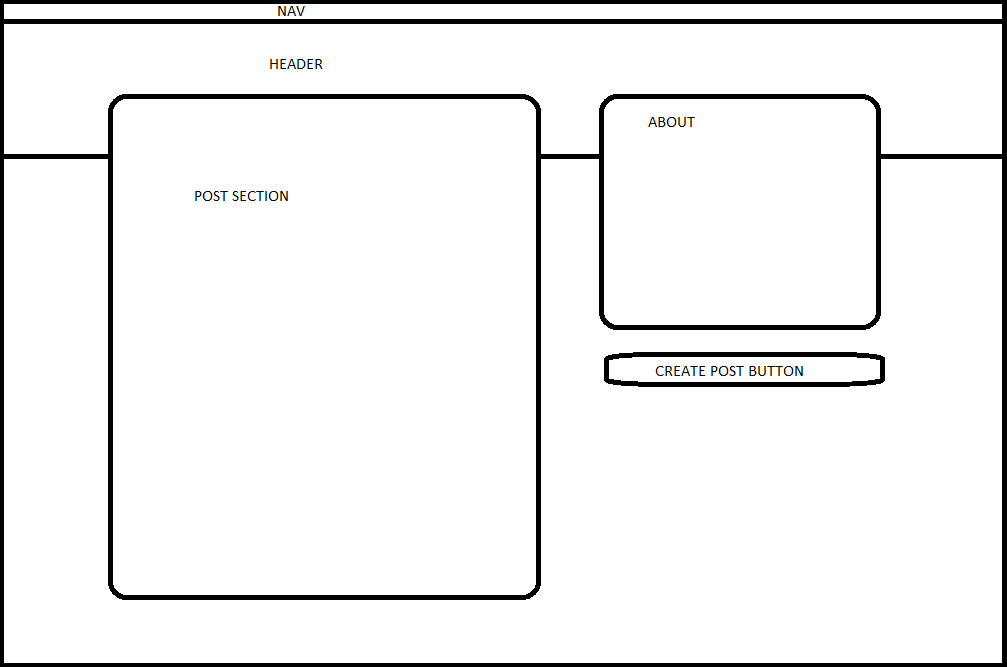
\includegraphics[width=60mm]{images/sketch.png}
    	\caption{Blog List Sketch}
    \end{figure}
	\begin{figure}[H]
  	  \centering
   	 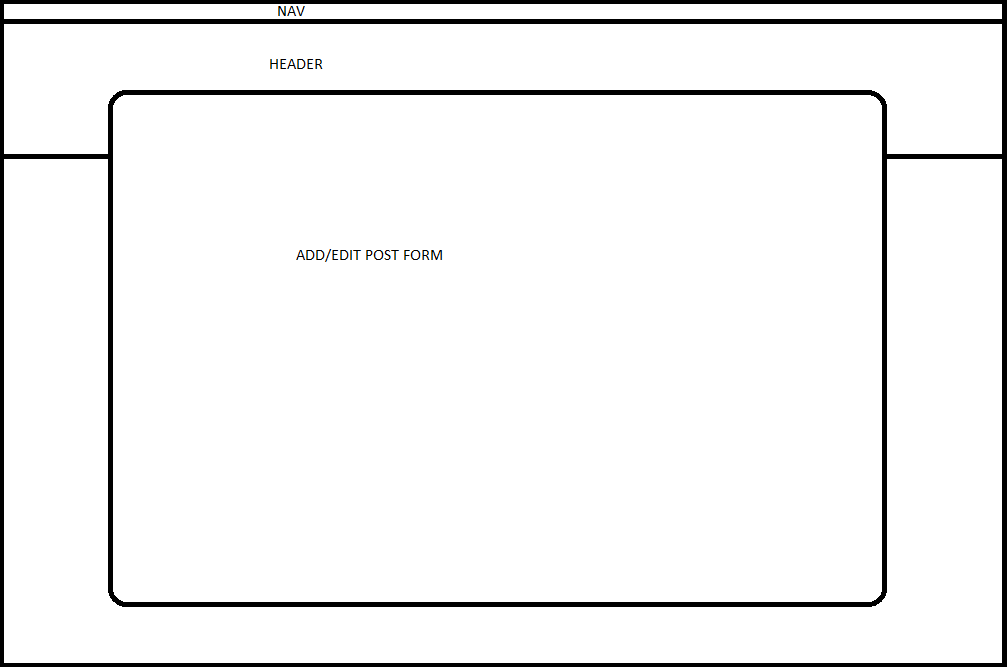
\includegraphics[width=60mm]{images/en_sketch.png}
    	\caption{Create/Add Post Sketch}
    \end{figure}
\subsection{Back to Top}
The design features a back to top button which appears when the user scrolls down. This is beneficial as blogs may become lengthy. This allows for the user to simply click the button to return to the page. 
	\section{Implementation}
	\subsection{Design Implementation}
	The website was implemented firstly be writing the HTML of the webpage. Boostrap will be used to create a grid like structure to enable containers within the application to be scalable and also fit neatly within the maximum dimensions of the webpage. This allows for runner space at the left and right of the page with 20 percent margin on each side to fit the application in the centre of the page. 
  
\subsubsection{Homepage}
    The homepage allows the central hub for the users interaction of the website.  Firstly, the homepage allows the viewing of the blog ordered by newest first.  Users can view the post title, content and the author who had written the post. 

The homepage also allows for users to create posts which will redirect the user to /blog/add where a post creation form is created.  Lastly, users can edit and delete posts from the homepage. The homepage layout can be viewed below.
\begin{figure}[H]
  	  \centering
   	 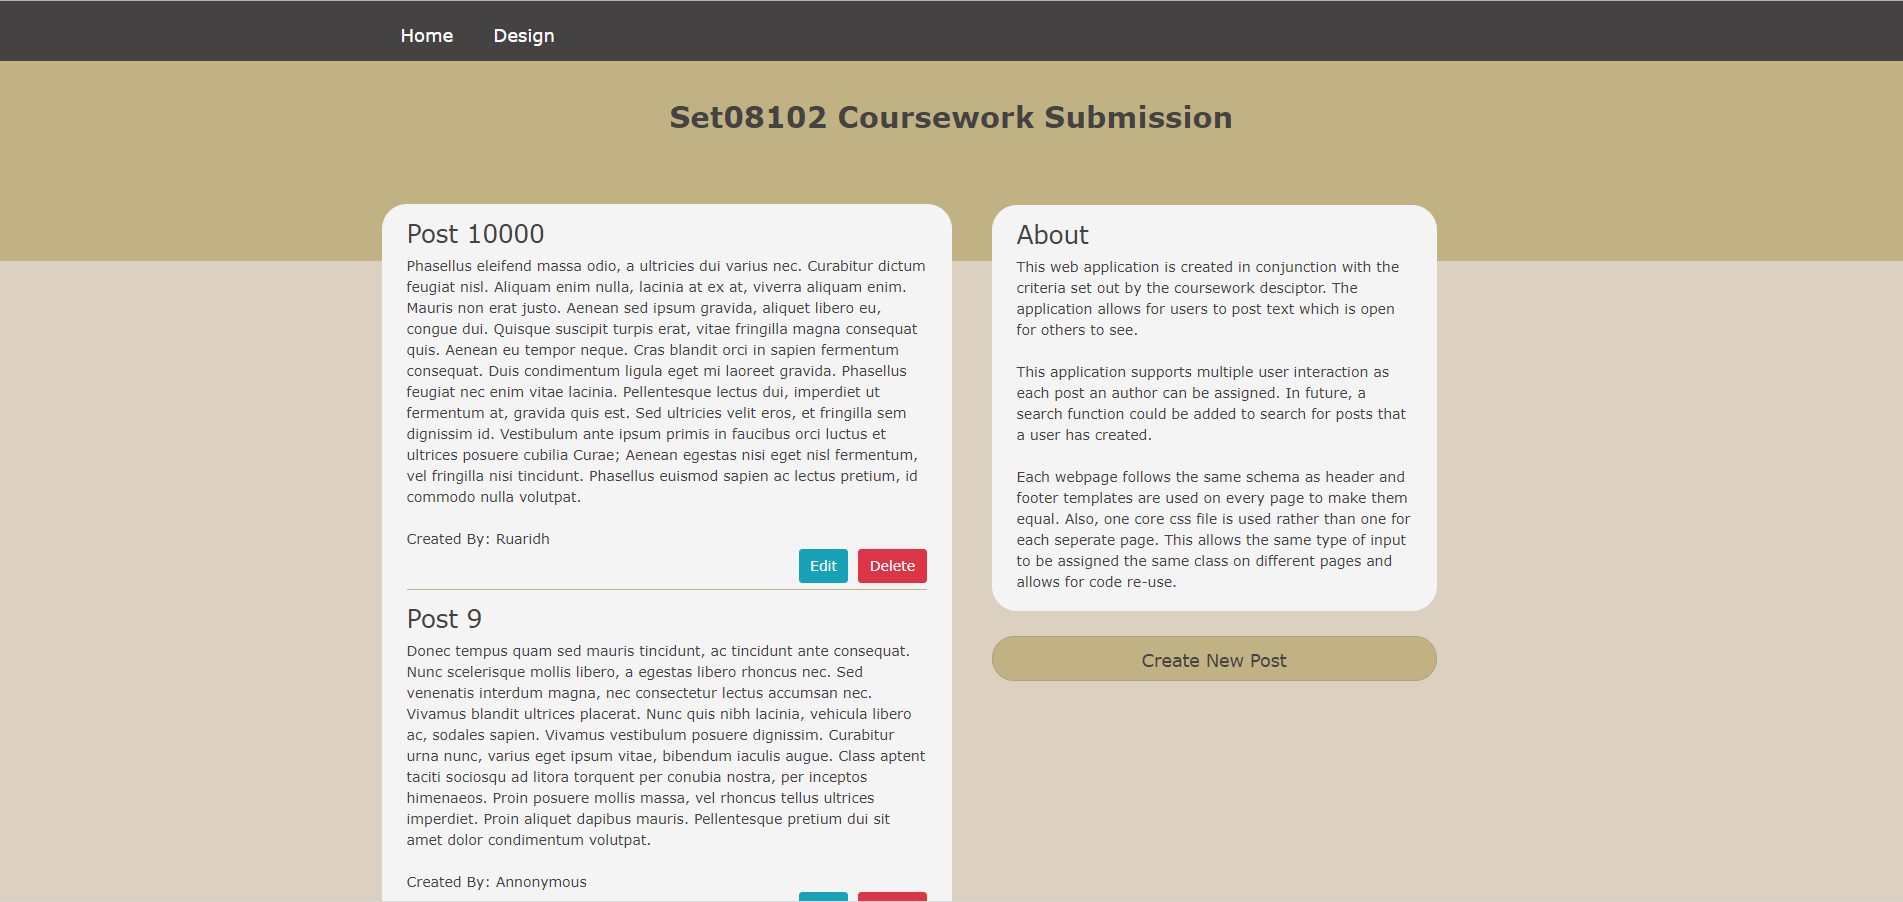
\includegraphics[width=100mm]{images/homepage.png}
    	\caption{Homepage}
    \end{figure} 
\subsubsection{Create Post}
The create post page allows user to create a post.  Within this page users can define a title, content and author of the post that is being created.  However, as this blog is openly shared with multiple users some data may be sensitive to the user and therefore by default users can post anonymously if no author is defined. 
\begin{figure}[H]
  	  \centering
   	 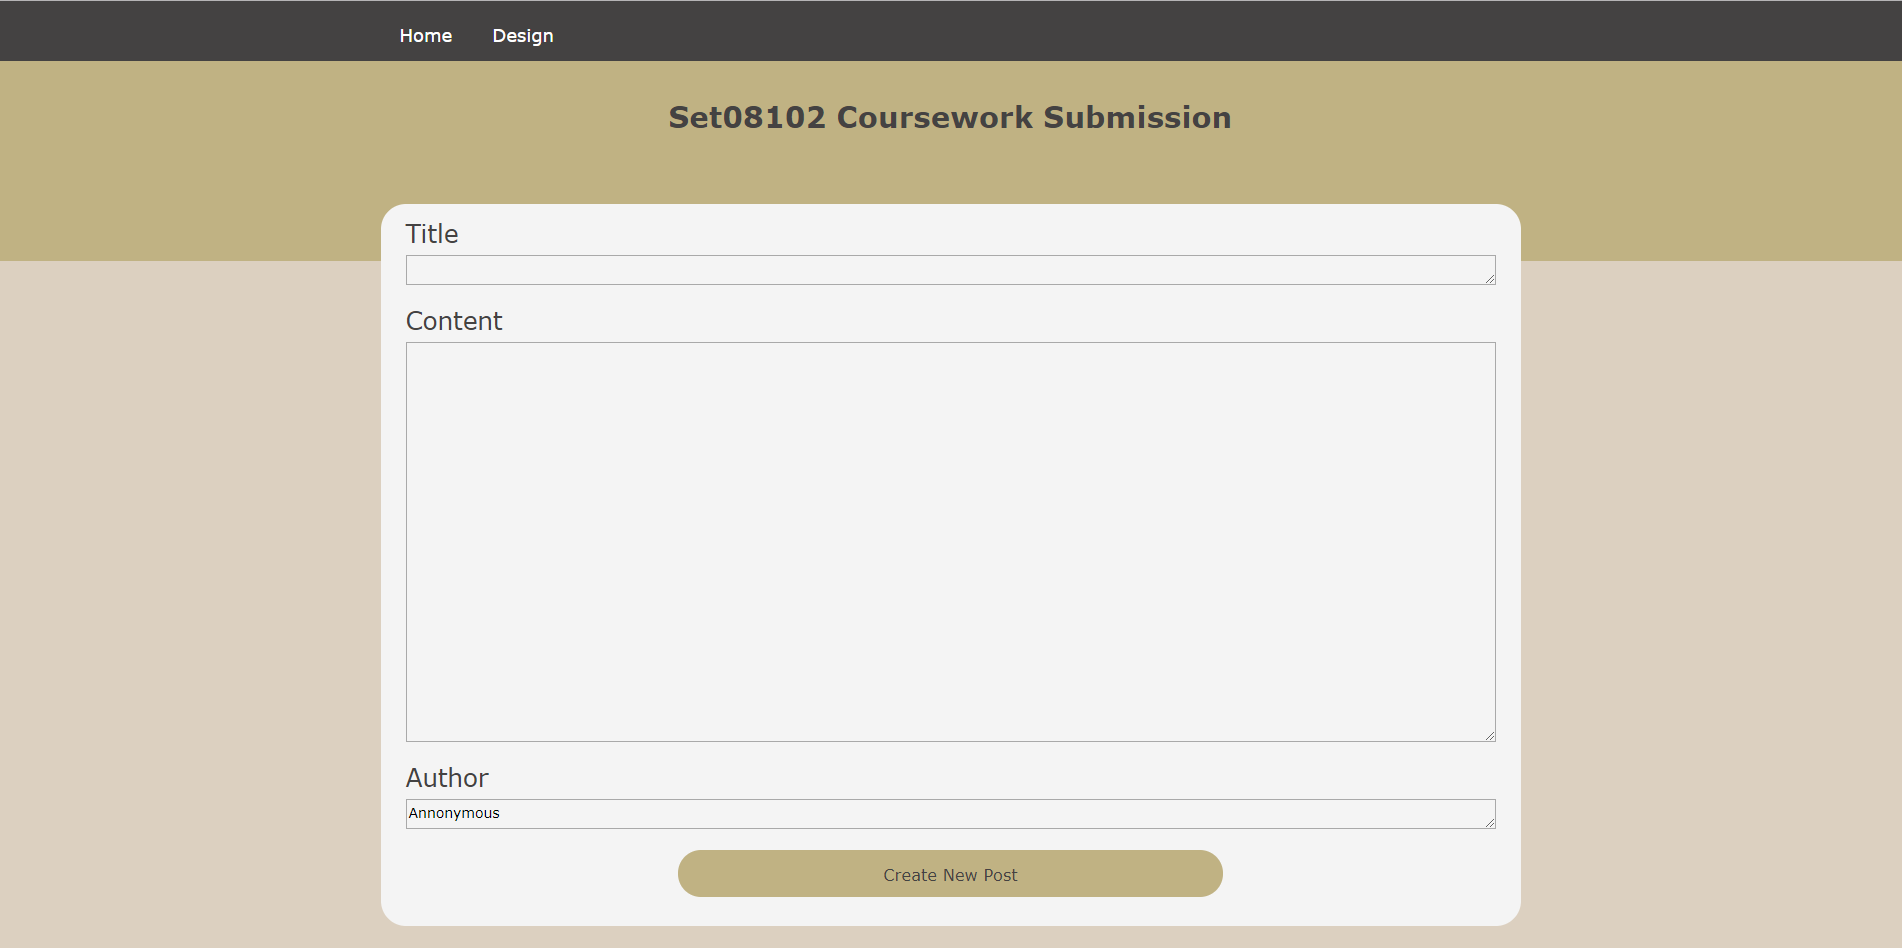
\includegraphics[width=100mm]{images/create.png}
    	\caption{Create Post}
 \end{figure} 
\subsubsection{Edit Post}
The edit post page allows users to edit a post.  This could be beneficial to fix spelling/grammar mistakes, update a post throughout the day or add extra information to a post.  For example, a user may post an issue they are having and once the issue is fixed put a notice at the top of the post. As seen in the create post section an author can defined.  However, within the edit page this cannot be editted. Once someone creates a post, I do not believe it should be able to be changed as the post belongs to that user. 
\begin{figure}[H]
  	  \centering
   	 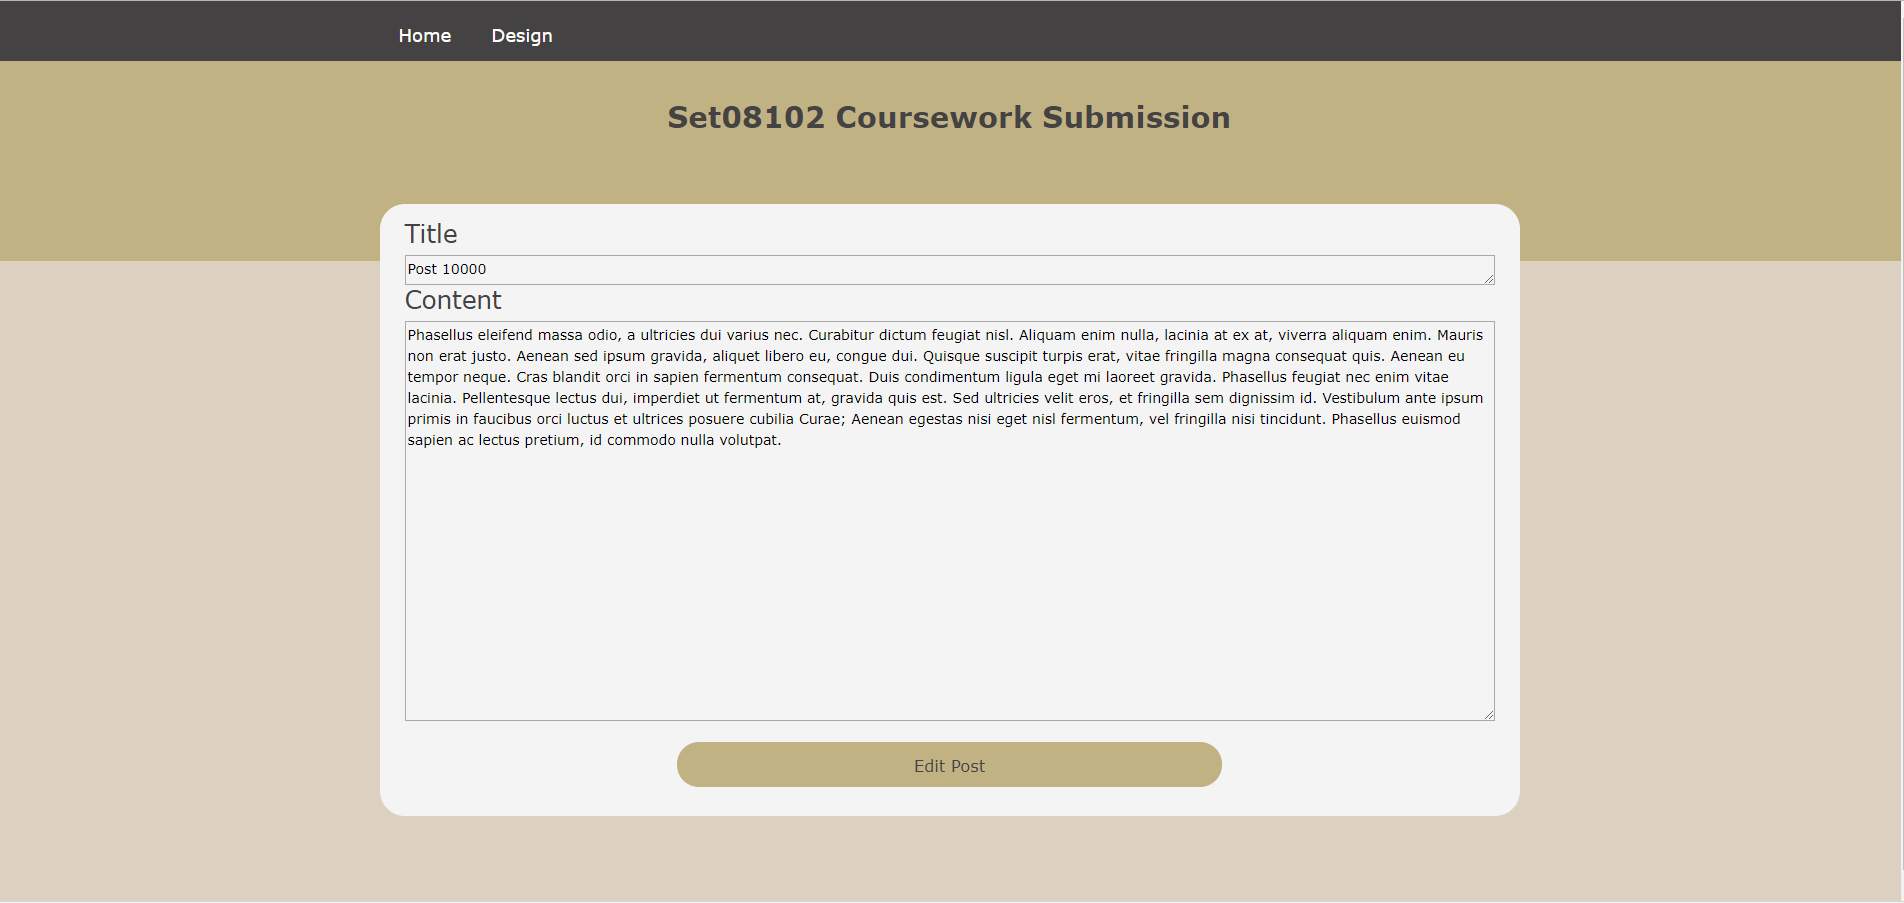
\includegraphics[width=100mm]{images/edit.png}
    	\caption{Edit Post}
 \end{figure} 

\subsection{Database}
Posts which the users create will be stored within a locally hosted MYSQL database which will allow queries to be ran to give the desired data output. \\

Data will be stored within the blog database and within the blog\_post table with the following structure;\\

\begin{center}
\begin{tabular}{c c c}
\textbf{Column} & \textbf{Datatype} & \textbf{Properties} \\
id & int(11) & auto increment,  PK\\
name & varchar(100) & NOT NULL \\
content & text & NOT NULL \\
author & varchar(40) & NOT NULL\\
\end{tabular}
\end{center}
Users will run CRUD queries on the database as described within the next section.
\subsection{CRUD Implementation}
CRUD is a terminology defined for users interaction with data.  This describes 4 basic methods users should be able to do with the data stored as described below;
\begin{itemize}
\item \textbf{C}reate
\item \textbf{R}ead 
\item \textbf{U}pdate 
\item \textbf{D}elete 
\end{itemize}

nodeJS is used for the backend server setup which will allow the user of the application  to be able to carry out 4 key requests to the server - GET, POST, PUT, DELETE. Each of these requests allow for CRUD to be carried out and are detailed in the following sub-sections. 
\subsubsection{Create}
To create a new blog post, a POST request is sent to the server with the data defined by the user. To allow the data to be attached to the POST two things must be setup.
\begin{enumerate}
\item Variable
A variable is set to the data which is to be stored within the database. The data is escaped to avoid an SQL Injection attack and also trimmed to take out extra spaces. The variable setup can be viewed in Listing 1: Variable Setup

\begin{lstlisting}[language=javascript,caption={Variable Setup}]
var bPost = {
            name: req.sanitize('name').escape().trim(),
            content: req.sanitize('content').escape().trim(),
            author: req.sanitize('author').escape().trim()
        }
\end{lstlisting}

\item Query
The database must be queried for the data to be inserted into the database.  This query will take take data stored within the above variable and insert it into the request (Listing 2: Create Query).
\begin{lstlisting}[language=javascript,caption={Create Query}]
req.getConnection(function(error, conn) \{
            conn.query('INSERT INTO blog_post SET ?', bPost,
        \}
\end{lstlisting}
\end{enumerate}

\subsubsection {Read}
To be able to read the post data which is stored in the database a GET request is made to the server.  This request fetches the data from the database and allows it to be printed to the database.  A query must be performed to the database for the relevant data to be retrieved (Listing 3: GET Query).
\begin{lstlisting}[language=SQL,caption={GET Query}]
SELECT * FROM blog_post
ORDER BY id DESC;
\end{lstlisting}

Although requesting a query to the database via a GET request this does not allow the data to be printed to the webpage.  A for loop using Embedded Javascript (EJS)is  used to read through read row of data and print it to page (Listing 4: Read For Loop)
\begin{lstlisting}[language=javascript,caption={Read For Loop}]
  <\% if (data) \{ \%>
          <\% data.forEach(function(bPost)\{ \%>
          <h3><\%= bPost.name \%><br /></h3>
          <\%= bPost.content \%><br /><br />
          Created By: <\%= bPost.author \%><br />
\end{lstlisting}
\subsubsection{Update}
Update uses a PUT request to the database with the updated data.  Much like Create a similar methods applies with using the bPost variable(Listing 1: Variable Setup). However, the author is excluded as this does not require to be updated. Also, a query must be sent to the database in order for the row to be updated (Listing 5: Update Query)

\begin{lstlisting}[language=javascript,caption={Update Query}]
  req.getConnection(function(error, conn) {
            conn.query('UPDATE blog_post SET ? WHERE id = ' + req.params.id, bPost,
\end{lstlisting}
\subsubsection{Delete}
Delete is similar to Create and Update however is more simpilar due to the only parameter required is the id of the post (Listing 6: Delete Variable).  
\begin{lstlisting}[language=javascript,caption={Delete Variable}]
 var del = \{ id: req.params.id \}
\end{lstlisting}
The delete sends a DELETE request to the database with what row to delete defined by the id of the post (Listing 7: Delete Query). 
\begin{lstlisting}[language=javascript,caption=\{Delete Query\}]
req.getConnection(function(error, conn) \{
        conn.query('DELETE FROM blog_post WHERE id = ' + req.params.id, del,
\end{lstlisting}

\section{Critical Evaluation}
\subsection{Requirements}
	The requirements of this webpage set out in Section 2.2 are displayed below with whether they have been completed or not.
	\subsubsection {Navigation}
	\begin{itemize}
	\item[\done] Placed on the top of every webpage.
	\item[\done] Allow users to access key points within the webpage.
	\item[\done] Provide feedback when hovering.
	\end{itemize}
	\subsubsection {Database Querying}
	\begin{itemize}
	\item[\done] Users must be able to CREATE posts.
	\item[\done] Users must be able to READ posts.
	\item[\done] Users must be able to UPDATE posts.
	\item[\done] Users must be able to DELETE posts.
	\end{itemize}
	\subsubsection {Users}
	\begin{itemize}
	\item[\done] One of more users must be supported within the application (Section 4.2)
	\end{itemize}
\subsection{Users}
As mentioned in section 4.1.3. users have been completed as desired by the requirements.  However, the implementation of users is not entirely 100\% legitimate. \\

Multiple users are supported due to the fact an author can be assigned to each individual post. This allows for multiple users to share their posts with each other and give each post a persona as a user. \\

Security is an issue with this implementation as there is no password protected information.  Every user can access everyones data and read everyones posts, some people may wish their post to be private.  Every user can edit and delete every post. Therefore, someone could write a heart wrenching post for someone else just to delete it.  Improvements of this will be discussed in section 4.3. Improvements. 
	
\subsection{Improvements}
As this application is supposed to be a blog a lot of features can be added to enhance the functionality of the blog. Listed below in each subsection is potential improvements that could be made to the blog. 
\subsubsection{Users}
As explained in section 4.2. Users are a big improvement which could be made to the blog.  A login system would enhance security and protect peoples posts and data. Within this login system an administrator account would be beneficial to maintain the user accounts.
\subsubsection{Individual Feeds}
Within the current design all posts are viewed together.  However, with the implementation of user accounts individual blogs can be created which will view only posts belonging to that user. However, a full listing of blogs could also be viewed by the user.  A psuedocode of this can be viewed in Listing 8: User Defined Posts.
\begin{lstlisting}[language=javascript,caption={User Defined Posts}]
var uID= {
            userID: req.sanitize('userID').escape().trim(),
        }

req.getConnection(function(error, conn) \{
        conn.query(SELECT FROM users WHERE userID = ' + req.params.id, uID,
\end{lstlisting}

\subsubsection{User Defined CSS}
Within modern day blogs users can make their blog layout personal to them.  With the implentation of Users Accounts the blog could have been more custom with user defined css which will allow the user to change the background colors, fonts and perhaps upload images for backgrounds.  

\subsubsection{Editable Posts}
Currently posts are crammed into the one block text.  An improvement of this would allow posts to be allow line breaks, bold, italic, font changes and file uploads for the post. 

\section{Person Evaluation}
Personally I feel this coursework was a challenge.  However, once I understood the basics it became easier to initiate the GET, POST, PUT and DELETE. The blog could have had much more functionality but as I struggled to implement user accounts a lot of my ideas could not be achieved. 

\bibliographystyle{ieeetr}
\bibliography{references}
		
\end{document}